\subsection{Déscription du mouvement}
\label{sec:description_mouvement}
\framecard{Déscription du mouvement}
\begin{frame}{Description du mouvement}
\only<1>{
\begin{center}
	\ighf{configuration_mapping}{50mm}
\end{center}
}
\only<2-3>{
	Vecteur position: cartographie des points matériels $M$ dans repère Euclidien $\mathcal{E}$ muni d'un repère (observateur) $\mathcal{R}=\pdp{\ibv[1],\ibv[2],\ibv[3]}$
	
	\beq{\pv=\vct{p}{}{}\pdp{M} \in \Omega_0,\quad \pv=\sum_{n=1}^{3}p_k\ibv[k]}{position} 
	
	\beq{\xv=\vct{f}{}{}\pptp \in \Omega_t,\quad\forall \pptp \in \pdp{\Omega_0,\mathbb{I}_t} }{xpu}
}
\only<2>{
	\begin{enumerate}
		\item Trajectoires: $\mathcal{T}\pdp{M}=\pbp{\xv, \exists t'\Big\vert\quad \xv=\vct{f}{}{}\pdp{\pv;t'}}$
		\item Caractériser petites changement de trajectoires en temps
		\item Caractériser petites changement de position en espace
		\item La matière ne peut pas disparaître
	\end{enumerate}
}
\only<3>{
	\vspace{-2mm}
	\begin{enumerate}
		\item \vct{f}{}{}: transformation injective (deux points matériels peuvent pas occuper le même volume) $ \vct{p}{1}{}\neq\vct{p}{2}{} \Rightarrow \vct{x}{1}{}\neq\vct{x}{2}{}$
		\item Il existe sa transformation inverse $\vct{g}{}{}:\Omega_t\to\Omega_0$
		\item $\vct{f}{}{}\in \mathcal{C}^1\pdp{\Omega_k,\Delta_T}$ (par morceaux en espace/temps)
		\item Le trièdre reste droit (matière ne peut pas disparaître): $ \det\pdp{\vct{e}{1}{},\vct{e}{2}{},\vct{e}{3}{}}>0 \Leftrightarrow\det\pdp{\ibv[1],\ibv[2],\ibv[3]}>0,\quad \vct{e}{k}{}=\vct{f}{}{}\pdp{\vct{i}{k}{},t}$
	\end{enumerate}
}
\end{frame}

\begin{frame}{Déplacement et Gradient}
\only<1>{
\ighf{configuration_gradient}{65mm}
}
\only<2>{
\begin{itemize}
	\item Vecteur déplacement:
	\beq{\uv\pptp=\xv\pptp-\pv=\vct{f}{}{}\pptp-\pv}{}
	\item Tenseur gradient de la transformation: \beq{\vct{dx}{}{}=\Fgrad.\vct{dp}{}{},\quad \vct{du}{}{}=\pdp{\Fgrad-\ID}.\vct{dp}{}{}}{dxFdp} 
\end{itemize}
	\textit{Les vecteurs tangents des matériaux cartographient les vecteurs tangents spatiaux via le gradient de déformation.}	
\beq{\Fgrad=\cartFgrad}{Fexp}
\beq{\Fgrad=\curvFgrad}{Fcurv}\\ \hspace{-2mm}\vspace{5mm} coordonnées curvilignes $\xi_i$
}
\end{frame}

\begin{frame}{Larges Déformations [Large Strains]}
\only<1>{
	\txb{122}{2}{12}{
		\begin{center}
			\ighf{configuration_green_lagrange}{55mm}
		\end{center}
	}
}
\only<2>{
	\txb{125}{0}{9}{
		\hspace{-2mm}
\begin{itemize}
	  \itemsep0em 
	\item Tenseur des déformations de Green-Lagrange:\vspace{-3mm} \beq{\Estrain=\FEstrain=\UEstrain}{Estrain}\vspace{-3mm}
		\item  Allongement de la fibre $\ell_p\vct{i}{p}{}$:
		\beq{\frac{\norm{\vct{dx}{}{}}^2-\norm{\vct{dp}{}{}}^2}{\norm{\vct{dp}{}{}}^2}=\frac{\ell_x^2-\ell_p^2}{\ell_p^2}=2\pscl{\vct{i}{p}{}}{\Estrain. \vct{i}{p}{}} = 2 \mathbb{E}_{pp} }{dx2dp2} \vspace{-3mm}
		\item Distorsion angulaire des fibres $\ell_{p1}\vct{i}{p1}{}$ $\ell_{p2}\vct{i}{p2}{}$:
	\vspace{-5mm}
		\beq{
			\begin{split}
			& \sin\pdp{\gamma_{x12}} =\sin\pdp{\frac{\pi}{2}-\alpha_{x12}}= \cos\pdp{\alpha_{x12}} =  \\
			& = \frac{\pscl{\pdp{2\Estrain+\ID}.\vct{i}{p1}{}}{\vct{i}{p2}{}}}{\sqrt{
					\pscl{\pdp{2\Estrain+\ID}.\vct{i}{p1}{}}{\vct{i}{p1}{}}
				}\sqrt{
					\pscl{\pdp{2\Estrain+\ID}.\vct{i}{p2}{}}{\vct{i}{p2}{}}	
		}}   = \frac{2\mathbb{E}_{12}+1}{\sqrt{\pdp{2\mathbb{E}_{11}+1}\pdp{2\mathbb{E}_{22}+1}}}
	\end{split}
}{sinEstrain}
	\end{itemize}
}
}
\end{frame}

\begin{frame}{\hypertarget{frame:NAN}{Transformation de surface/volume}}
Formule de Nanson \textcolor{blue}{[NAN]}:
\ighf{nanson}{55mm}
\end{frame}

\begin{frame}{\hypertarget{frame:NAN}{Transformation de surface/volume}}
Formule de Nanson \textcolor{blue}{[NAN]}:
\setcounter{equation}{9}

\begin{itemize}
	\item Variation locale de volume $dV_0 = \pscl{\dpv[1] \wedge \dpv[2]}{\dpv[3]}$:\\
	$dv_t =\pscl{\dxv[1] \wedge \dxv[2]}{\dxv[3]}= \pscl{\Fgrad.\dpv[1] \wedge \Fgrad.\dpv[2]}{\Fgrad.\dpv[3]}$
	\beq{dv_t = det\pdp{\Fgrad} dV_0}{dVolJ} (propriété 4 de \vct{f}{}{}: le trièdre doit rester droit! $J=det\pdp{\Fgrad}$)

	% \item Variation locale de surface $dS_0\Nv = \dpv[1] \wedge \dpv[2]$:
	% \beq{ds_t\nv = \dxv[1]\wedge\dxv[2]= \Fgrad.\dpv[1]\wedge\Fgrad.\dpv[2] =dS_0 det\pdp{\Fgrad}\FgradTinv\Nv}{dS}

	
\end{itemize}
\end{frame}

\begin{frame}{\hypertarget{frame:NAN}{Transformation de surface/volume}}
Formule de Nanson \textcolor{blue}{[NAN]}:

\begin{itemize}
	\item Variation locale de surface $ds_0\nv(\pv,0) = \dpv[1] \wedge \dpv[2]$:\\
	$ds_t =\pscl{\dxv[1] \wedge \dxv[2]}{\nv\pxtp}= \pscl{\Fgrad.\dpv[1] \wedge \Fgrad.\dpv[2]}{\nv\pxtp}=det\pdp{\Fgrad}\pscl{\dpv[1] \wedge \dpv[2]}{\Fgradinv\nv\pxtp}=det\pdp{\Fgrad}ds_0\pscl{\FgradTinv.\nv(\pv,0)}{\nv\pxtp}$

	\beq{ds_t\nv\pxtp = ds_0 det\pdp{\Fgrad}\FgradTinv\nv\pdp{\pv,0}}{dS}

	
\end{itemize}
\end{frame}



\begin{frame}{Petites Déformations [Small Strains]}
\txb{110}{0}{11}{
\begin{itemize}
	\item Petits déplacements/Petites déformations:	\beq{\max_{\pxtp}\norm{\uv} \ll \mathcal{L} \pdp{\xv\approx\pv},  \max_{\pxtp}\norm{\gradt{u}{p}}^2=\max_{\pxtp}\gradpUT:\gradpU \ll 1}{petitDepDef} 
	\item Tenseur des petites déformations:
	\beq{\Estrain\approx\strain=\frac{1}{2}\pdp{\gradt{u}{x}+\gradtT{u}{x}} =\cartEspilon}{smallStrain}
	 $$\frac{\Delta \ell}{\ell_p} = \pscl{\vct{i}{p}{}}{\depsil \vct{i}{p}{}}=\depsil_{pp},\quad \frac{\Delta\gamma_{12}}{2}=\pscl{\vct{i}{1}{}}{\depsil \vct{i}{2}{}}=\depsil_{12}$$
	 \item Variation locale de volume:
	 {\scriptsize
	 \beq{\evol=\frac{\Delta v_t}{V_0}=\frac{\ell_{p1}+\Delta \ell_1}{\ell_{p1}}\frac{\ell_{p2}+\Delta \ell_2}{\ell_{p2}}\frac{\ell_{x3}+\Delta \ell_{p3}}{\ell_{p3}}\approx \frac{\Delta \ell_1}{\ell_{p1}}+ \frac{\Delta \ell_2}{\ell_{p2}}+\frac{\Delta \ell_{p3}}{\ell_{p3}}\approx Tr\pdp{\depsil}}{epsvol}\\ \vspace{-2mm}
 $\Delta \ell_{pi}= o\pdp{\ell_{pi}}$}
\end{itemize}
}
\txb{15}{110}{11}{
\igwf{small-displ}{10mm}
}
\end{frame}


\begin{frame}{Théorème de la divergence }
\txb{120}{0}{11}{
	\centering
	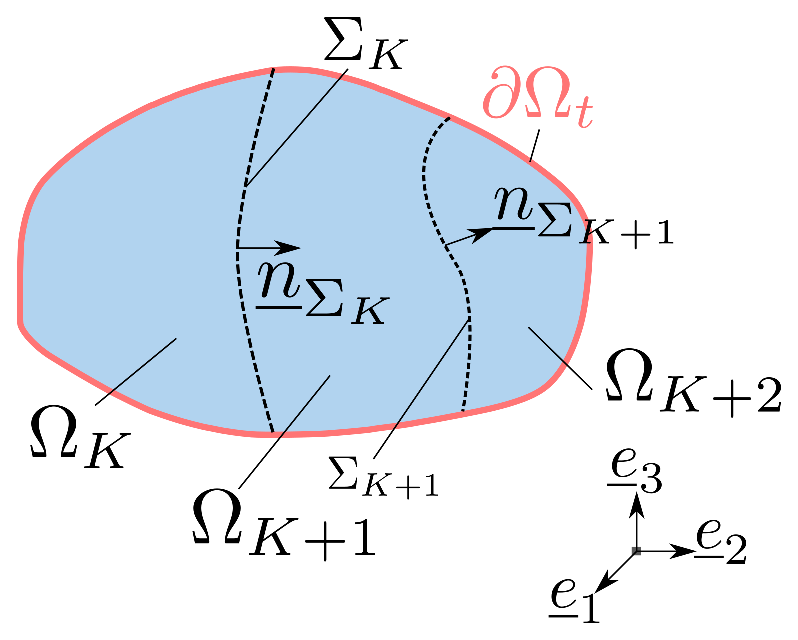
\includegraphics[height=65mm]{divergence_multiple_discontinuities}
	$\nv[\Sigma_K]$: sortant de $K$ et entrant dans $K+1$
}
\end{frame}

\begin{frame}{Théorème de la divergence}
	\txb{120}{0}{11}{
		\itmz{
			\item Théorème classique:
			$$ \int_{\partial\Omega_i(t) } \At[i].\nv[i]\pxtp ds =\int_{\Omega_i(t)} \divergence \At[i]\pxtp dv\quad \forall \Omega_{i}(t)$$
			avec $\nv[i]$ sortant de $\Omega_{i(t)}$
			\item<2-> Sur $\Omega(t)=\cup_i \Omega_i(t)$, avec discontinuités internes $\Sigma_K$ de $\At$:
			\itmz{
				\item<3->  $\sum_i\int_{\partial\Omega_i(t) } \At.\nv\pxtp ds = \sum_i\int_{\Omega_i(t)} \divergence \At[i]\pxtp dv = \int_{\Omega} \divergence \At dv $
				\item<4-> $\sum_i\int_{\partial\Omega_i(t) } \At[i].\nv[i]\pxtp ds = \sum_{j}\int_{\partial\Omega_j(t)\cap\partial\Omega(t) } \At[j].\nv[j] ds + \sum_{K}\int_{\Sigma_K(t)} \pdp{\At[K]-\At[K+1]}.\nv[\Sigma_K] ds=$\\ 
				$\int_{\partial\Omega(t)} \At.\nv ds - \sum_{K}\int_{\Sigma_K(t)} \disc{\At}.\nv[\Sigma_K] ds$
				\item<5->
				\hspace{-5mm}\beq{\int_{\Omega} \divergence \At dv = \int_{\partial\Omega(t) } \At.\nv\pxtp ds -\sum_{K}\int_{\Sigma_K(t)} \disc{\At}.\nv[\Sigma_K] ds}{div_theo}
			}
		}
	
}
\end{frame}


\begin{frame}{Théorème du transport [Reynolds theorem]}
\txb{120}{0}{11}{
	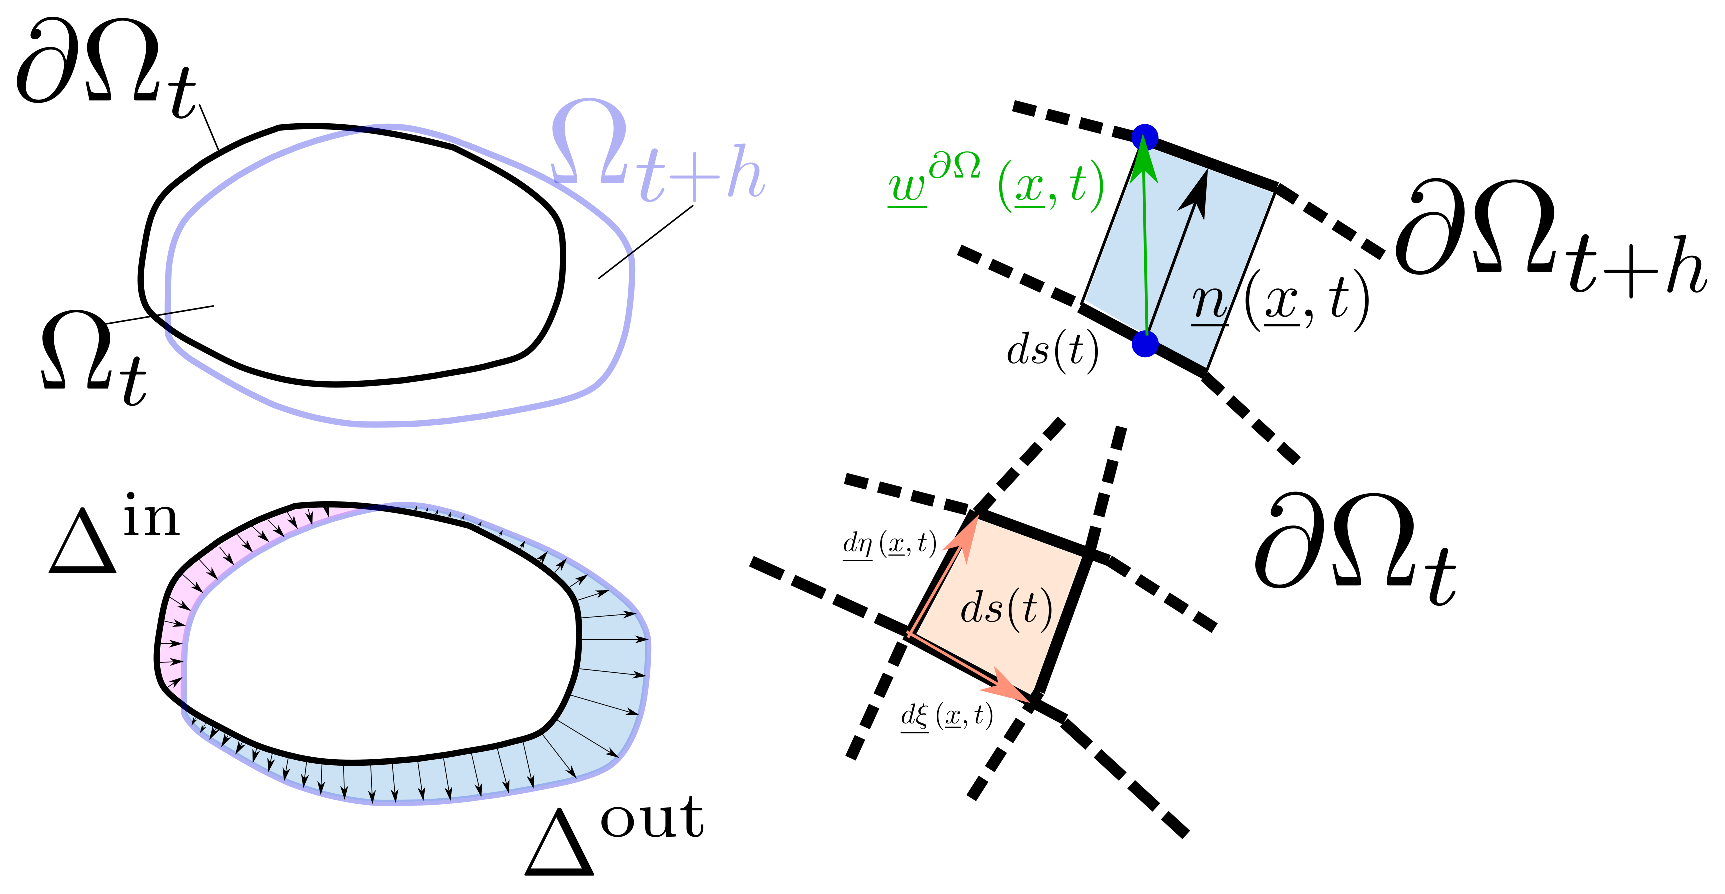
\includegraphics[height=65mm]{transport_theorem}
}
\end{frame}

\begin{frame}{Théorème du transport [Reynolds theorem]}
\txb{120}{0}{11}{
\begin{itemize}
	\item Théorème du transport \hypertarget{frame:TTR}{\textcolor{blue}{[TTR]}}: $\forall \Omega_t,\Sigma$ et $\forall \tens{b}{}{}\pxtp$
	\beq{\matd\int_{\Omega_t} \tens{b}{}{}  dv_t = \int_{\Omega_t}\pdp{ \partdt[\tens{b}{}{}]+\divergence\pdp{\tens{b}{}{}\otimes\vV} }dv_t+\int_{\Sigma\cap\Omega_t}\disc{ \tens{b}{}{}\otimes \pdp{\vct{v}{}{}-\vct{v}{\Sigma}{}}}.{\nvsigma}ds_t }{theo_transp}
	\begin{center}
		\ighf{patate_disc}{25mm} $\disc{\alpha}=\alpha^\text{\circled{2}}-\alpha^\text{\circled{1}}$	
	\end{center}	
\end{itemize}
}
\txb{123}{2}{68}{
	Surface de discontinuité $\Sigma$ du champs $\tens{b}{}{}\pxtp$, se propageant à vitesse $\vV[\Sigma]$\vspace{-4mm}
	\begin{itemize}
		\itemsep0em
		\item $\partdt[\tens{b}{}{}]$: variation en temps, à volume $\Omega_t$ figé
		\item $\divergence\pdp{\tens{b}{}{}\otimes\vV}$: mouvement point matériel + variation  volume $\Omega_{t}$ ($\divergence\vV$)
		\item $\disc{\tens{b}{}{}\otimes \pdp{\vV-\vV[\Sigma]}}.{\nvsigma}$ variation due au mouvement de $\Sigma$
	\end{itemize}
}
\end{frame}